% Options for packages loaded elsewhere
\PassOptionsToPackage{unicode}{hyperref}
\PassOptionsToPackage{hyphens}{url}
%
\documentclass[
  12pt,
]{article}
\usepackage{lmodern}
\usepackage{amsmath}
\usepackage{ifxetex,ifluatex}
\ifnum 0\ifxetex 1\fi\ifluatex 1\fi=0 % if pdftex
  \usepackage[T1]{fontenc}
  \usepackage[utf8]{inputenc}
  \usepackage{textcomp} % provide euro and other symbols
  \usepackage{amssymb}
\else % if luatex or xetex
  \usepackage{unicode-math}
  \defaultfontfeatures{Scale=MatchLowercase}
  \defaultfontfeatures[\rmfamily]{Ligatures=TeX,Scale=1}
\fi
% Use upquote if available, for straight quotes in verbatim environments
\IfFileExists{upquote.sty}{\usepackage{upquote}}{}
\IfFileExists{microtype.sty}{% use microtype if available
  \usepackage[]{microtype}
  \UseMicrotypeSet[protrusion]{basicmath} % disable protrusion for tt fonts
}{}
\makeatletter
\@ifundefined{KOMAClassName}{% if non-KOMA class
  \IfFileExists{parskip.sty}{%
    \usepackage{parskip}
  }{% else
    \setlength{\parindent}{0pt}
    \setlength{\parskip}{6pt plus 2pt minus 1pt}}
}{% if KOMA class
  \KOMAoptions{parskip=half}}
\makeatother
\usepackage{xcolor}
\IfFileExists{xurl.sty}{\usepackage{xurl}}{} % add URL line breaks if available
\IfFileExists{bookmark.sty}{\usepackage{bookmark}}{\usepackage{hyperref}}
\hypersetup{
  pdftitle={Supplementary Information},
  hidelinks,
  pdfcreator={LaTeX via pandoc}}
\urlstyle{same} % disable monospaced font for URLs
\usepackage[margin=1in]{geometry}
\usepackage{longtable,booktabs}
\usepackage{calc} % for calculating minipage widths
% Correct order of tables after \paragraph or \subparagraph
\usepackage{etoolbox}
\makeatletter
\patchcmd\longtable{\par}{\if@noskipsec\mbox{}\fi\par}{}{}
\makeatother
% Allow footnotes in longtable head/foot
\IfFileExists{footnotehyper.sty}{\usepackage{footnotehyper}}{\usepackage{footnote}}
\makesavenoteenv{longtable}
\usepackage{graphicx}
\makeatletter
\def\maxwidth{\ifdim\Gin@nat@width>\linewidth\linewidth\else\Gin@nat@width\fi}
\def\maxheight{\ifdim\Gin@nat@height>\textheight\textheight\else\Gin@nat@height\fi}
\makeatother
% Scale images if necessary, so that they will not overflow the page
% margins by default, and it is still possible to overwrite the defaults
% using explicit options in \includegraphics[width, height, ...]{}
\setkeys{Gin}{width=\maxwidth,height=\maxheight,keepaspectratio}
% Set default figure placement to htbp
\makeatletter
\def\fps@figure{htbp}
\makeatother
\setlength{\emergencystretch}{3em} % prevent overfull lines
\providecommand{\tightlist}{%
  \setlength{\itemsep}{0pt}\setlength{\parskip}{0pt}}
\setcounter{secnumdepth}{5}
\usepackage{rotating}
\usepackage{setspace}
\usepackage{booktabs}
\usepackage{longtable}
\usepackage{array}
\usepackage{multirow}
\usepackage{wrapfig}
\usepackage{float}
\usepackage{colortbl}
\usepackage{pdflscape}
\usepackage{tabu}
\usepackage{threeparttable}
\usepackage{threeparttablex}
\usepackage[normalem]{ulem}
\usepackage{makecell}
\usepackage{xcolor}
\ifluatex
  \usepackage{selnolig}  % disable illegal ligatures
\fi
\newlength{\cslhangindent}
\setlength{\cslhangindent}{1.5em}
\newlength{\csllabelwidth}
\setlength{\csllabelwidth}{3em}
\newenvironment{CSLReferences}[2] % #1 hanging-ident, #2 entry spacing
 {% don't indent paragraphs
  \setlength{\parindent}{0pt}
  % turn on hanging indent if param 1 is 1
  \ifodd #1 \everypar{\setlength{\hangindent}{\cslhangindent}}\ignorespaces\fi
  % set entry spacing
  \ifnum #2 > 0
  \setlength{\parskip}{#2\baselineskip}
  \fi
 }%
 {}
\usepackage{calc}
\newcommand{\CSLBlock}[1]{#1\hfill\break}
\newcommand{\CSLLeftMargin}[1]{\parbox[t]{\csllabelwidth}{#1}}
\newcommand{\CSLRightInline}[1]{\parbox[t]{\linewidth - \csllabelwidth}{#1}\break}
\newcommand{\CSLIndent}[1]{\hspace{\cslhangindent}#1}

\title{Supplementary Information}
\author{}
\date{\vspace{-2.5em}}

\begin{document}
\maketitle

{
\setcounter{tocdepth}{2}
\tableofcontents
}
\pagenumbering{gobble}
\pagenumbering{arabic}
\doublespacing

\hypertarget{changes-in-covered-counties}{%
\section*{Changes in Covered Counties}\label{changes-in-covered-counties}}
\addcontentsline{toc}{section}{Changes in Covered Counties}

\begin{singlespace}
\begin{table}[!h]

\caption{\label{tab:change-tab}\label{tab:table-changes} Changes in Covered Counties}
\centering
\begin{tabular}[t]{lcccccc}
\toprule
\multicolumn{1}{c}{ } & \multicolumn{3}{c}{Polling Places} & \multicolumn{3}{c}{Early Voting Days} \\
\cmidrule(l{3pt}r{3pt}){2-4} \cmidrule(l{3pt}r{3pt}){5-7}
County & Actual & Expected & Share Open & 2018 & 2016 & Change\\
\midrule
Bay & 6 & 44 & 13.6\% & 10 & 9 & 1\\
Calhoun & 6 & 6 & 100.0\% & 15 & 13 & 2\\
Franklin & 8 & 7 & 114.3\% & 10 & 8 & 2\\
Gadsden & 25 & 25 & 100.0\% & 15 & 13 & 2\\
Gulf & 2 & 10 & 20.0\% & 10 & 8 & 2\\
Jackson & 3 & 14 & 21.4\% & 10 & 13 & -3\\
Liberty & 7 & 7 & 100.0\% & 13 & 13 & 0\\
Washington & 4 & 12 & 33.3\% & 8 & 13 & -5\\
\bottomrule
\end{tabular}
\end{table}
\end{singlespace}

\hypertarget{impact-on-registrations}{%
\section*{Impact on Registrations}\label{impact-on-registrations}}
\addcontentsline{toc}{section}{Impact on Registrations}

As discussed in the body of this paper, our estimates all test the effect of the hurricane on turnout as a share of registered voters. This probably leads to an underestimation of the treatment effect. As Figure \ref{fig:pre-deadline} makes clear, the number of registrations in the weeks before the election in the treated counties was substantially lower than we might have expected based on the rest of the state.\footnote{Because the storm impacted the registration deadline in some of the treated counties in 2018, we plot the total number of registrations in the 5 weeks prior to election day each year.} Because our estimates exclude the individuals who would have registered and voted in the absence of the storm, our estimated treatment effects are likely highly conservative.

\begin{figure}[H]

{\centering 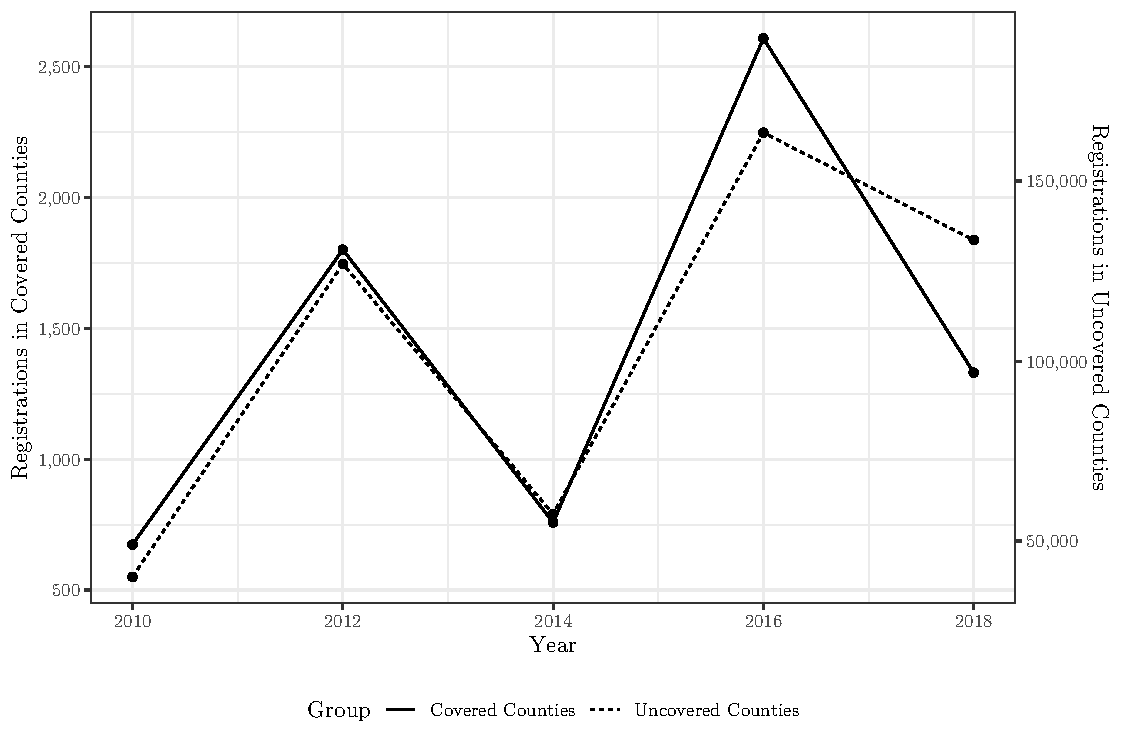
\includegraphics{si_files/figure-latex/regs-chunk-1} 

}

\caption{\label{fig:pre-deadline}Registrations in Final Weeks Before Election}\label{fig:regs-chunk}
\end{figure}

\hypertarget{alternative-processing-approaches-for-ame}{%
\section*{Alternative Processing Approaches for AME}\label{alternative-processing-approaches-for-ame}}
\addcontentsline{toc}{section}{Alternative Processing Approaches for AME}

In the body of the paper, we use nearest-neighbor matching and a genetic weighting process. Here, we demonstrate that our primary results are robust to a variety of different pre-processing approaches.

In model 1 of Table \ref{tab:alt-specs} we do not process the data in any way before running a difference-in-differences model. In other words, every treated voter and potential control voter is included once, and all voters receive a weight of 1. This is a formalization of the left-hand panel of Figure 2{[}HARD CODED---CONFIRM BEFORE SUBMISSION{]} in the body of the paper.

In model 2, we use an approach called entropy balancing (\protect\hyperlink{ref-Hainmueller2012}{Hainmueller 2012}). In this approach, every treated voter is given a weight of 1, while every control voter receives a unique weight based on their sociodemographic characteristics and past turnout history. Balancing is done using the same covariates used for the primary match in the body of the manuscript.

In model 3, we use propensity score matching (\protect\hyperlink{ref-Caliendo2008}{Caliendo and Kopeinig 2008}). Each voter's propensity score is calculated using the same covariates as in the body of the paper. After estimating each voter's propensity score, we use a nearest-neighbor matching approach. Each treated voter is matched with 5 controls. Matching is done with replacement, and ties are randomly broken.

In model 4, we match treated voters to 5 controls using only individual-level characteristics (race, gender, party affiliation, age, and historical turnout). Control voters must exactly match their treated voters; treated voters who do not exactly match any control voters are dropped. Once again, matching is done with replacement, and ties are randomly broken.

Finally, in model 5, we allow for unique time trends over the 2010--2018 period for each county in the state. Here, we use the same matches as those produced in the body of the paper, but interact each voter's county with a running variable for time.

As a reminder, the estimated treatment effect from the body of the paper was -6.6 percentage points. Table \ref{tab:alt-specs} makes clear that our results are robust to a variety of preprocessing and approaches. Entropy balancing and propensity score matching return estimated effects within 0.1 percentage points of our primary models, as does the model including county-linear time trends. Exact matching and unprocessed difference-in-difference approaches return substantially larger treatment effects.

\begin{singlespace}
\input{"../temp/rob_clean.tex"}
\end{singlespace}

\hypertarget{county-specific-effects}{%
\section*{County-Specific Effects}\label{county-specific-effects}}
\addcontentsline{toc}{section}{County-Specific Effects}

In the body of this paper, Figure 2 presents the overall pre- and post-treatment trends for treated and control voters. However, lumping each of the treated counties together masks considerable heterogeneity. In Figure \ref{fig:ind-counties} we plot the unprocessed and matched turnout trends for treated and control voters, broken out for each of the 8 treated counties. Figure \ref{fig:ind-counties} makes clear that the treatment effect varied substantially by county.

\begin{figure}[H]

{\centering 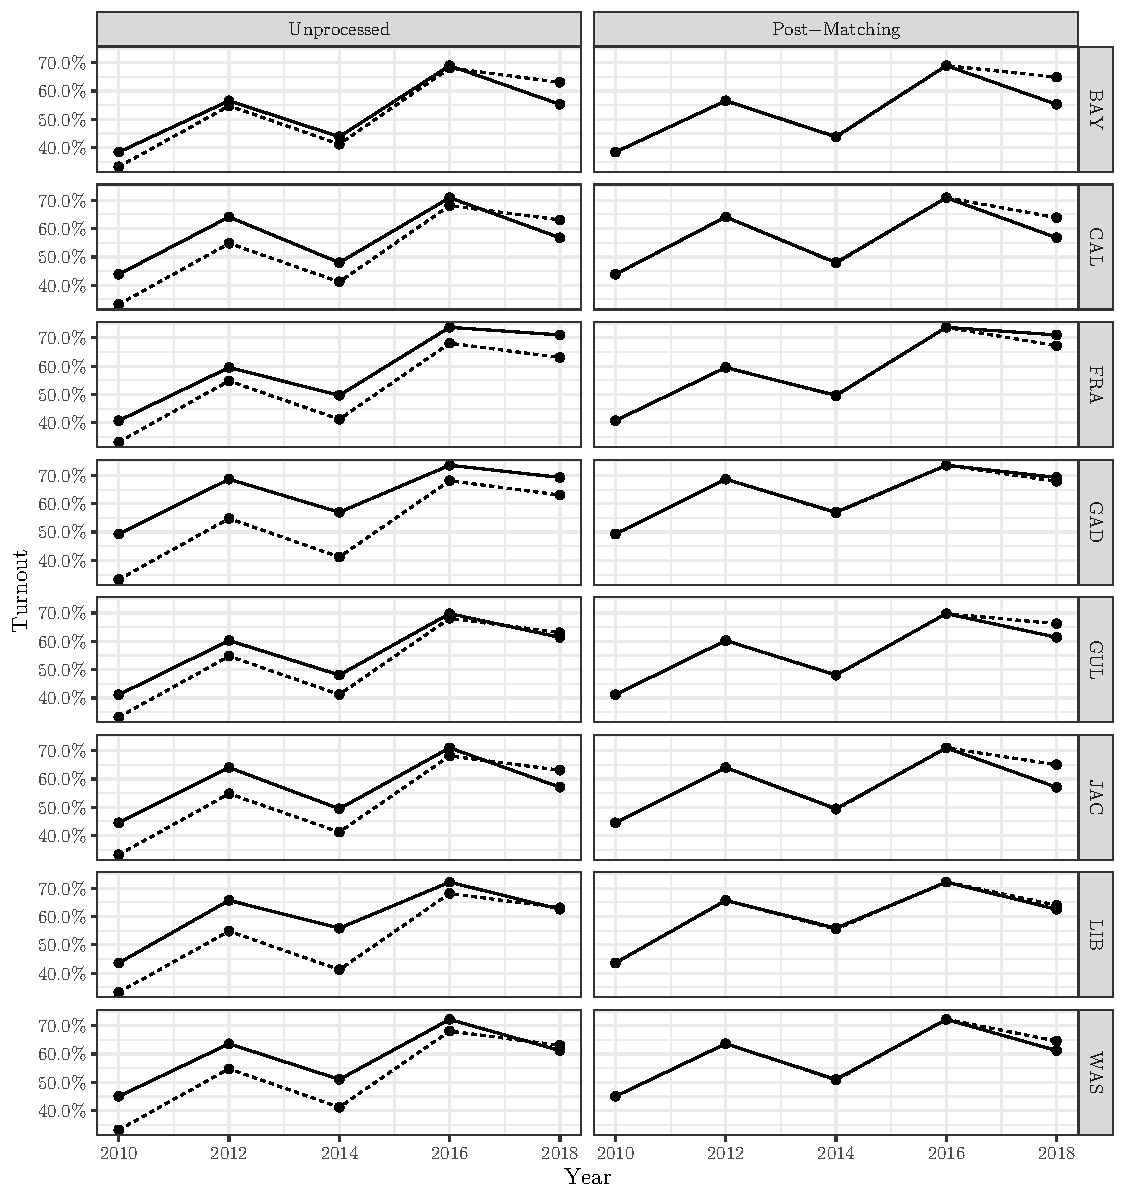
\includegraphics{si_files/figure-latex/indcs-chunk-1} 

}

\caption{\label{fig:ind-counties}Pre- and Post-Matching County Plots}\label{fig:indcs-chunk}
\end{figure}

Table \ref{tab:county-effs} re-estimates model 1 from Table 2 in the body of the paper, but interacts the treatment term with each of the treated counties. This allows us to measure the difference in treatment effect for each county. The reference category in Table \ref{tab:county-effs} is Bay County.

\begin{singlespace}
\input{"../temp/county_clean_regs.tex"}
\end{singlespace}

As discussed in the body of the paper we argue that the treatment effects are largely moderated by the number of polling places each county kept open, and that these effects were larger than the relative rainfall. In Figures \ref{fig:rain-counties} and \ref{fig:inter-counties}, we plot each county's estimated treatment effect from Table \ref{tab:county-effs} against the relative rainfall experienced by the average voter in each county, and share of polling places that county kept open. The line of best fit is weighted by the number of registered voters in each county. The relationship is clear: while there is not a particularly strong relationship between county rainfall and the estimated treatment effect, the treatment effect was much larger in counties where more polling places were closed.

\begin{figure}[H]

{\centering 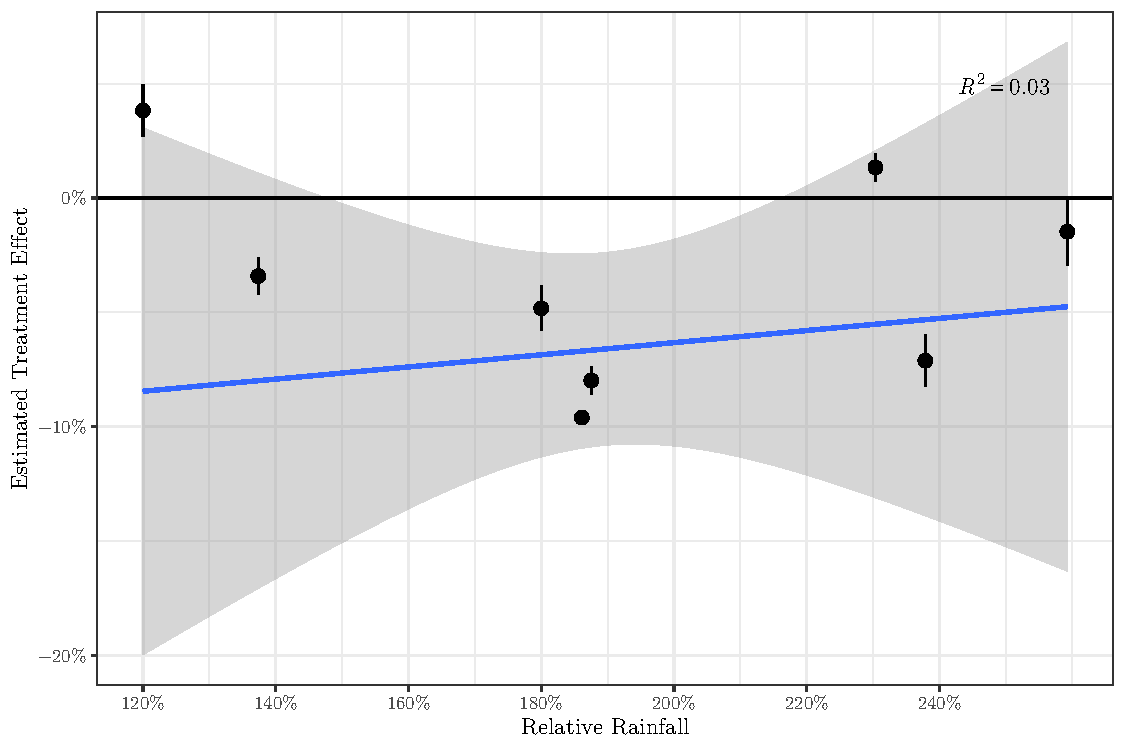
\includegraphics{si_files/figure-latex/rain-chunk-1} 

}

\caption{\label{fig:rain-counties}Relationship Between County Treatment Effect and Relative Rainfall}\label{fig:rain-chunk}
\end{figure}

\begin{figure}[H]

{\centering 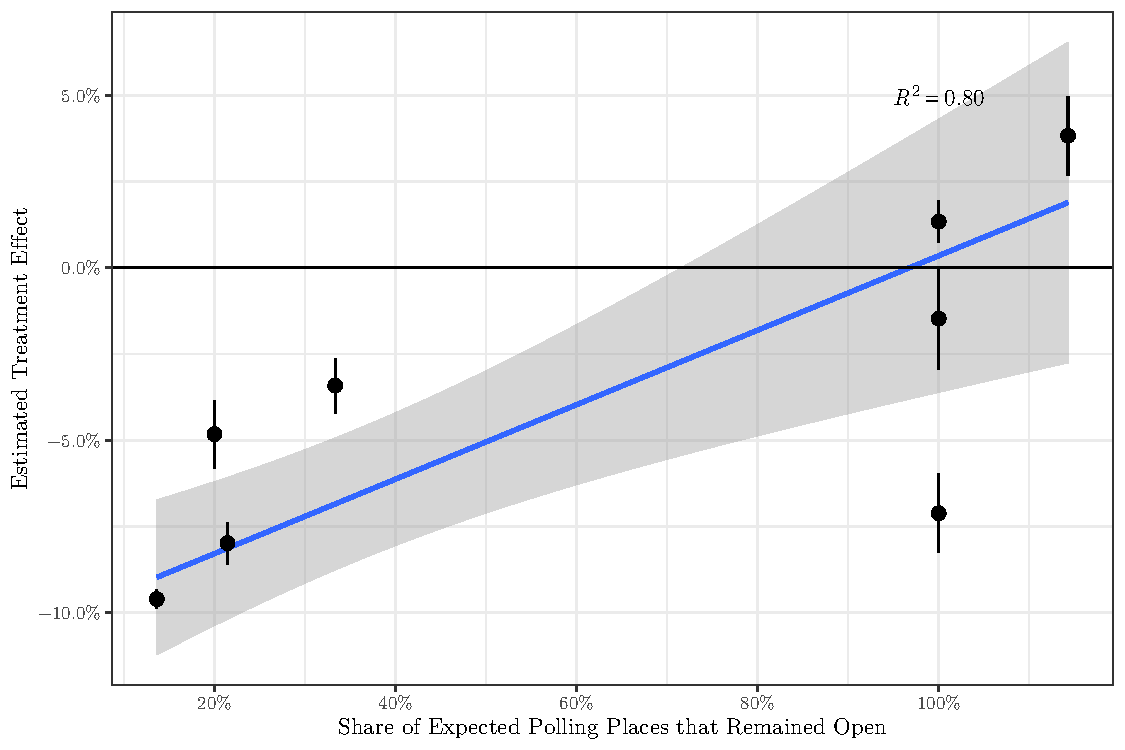
\includegraphics{si_files/figure-latex/inter-chunk-1} 

}

\caption{\label{fig:inter-counties}Relationship Between County Treatment Effect and Share of Polling Places Open}\label{fig:inter-chunk}
\end{figure}

\hypertarget{alternative-processing-approaches-for-triple-differences-model}{%
\section*{Alternative Processing Approaches for Triple-Differences Model}\label{alternative-processing-approaches-for-triple-differences-model}}
\addcontentsline{toc}{section}{Alternative Processing Approaches for Triple-Differences Model}

In the body of this manuscript we match pairs of voters on either side of the administrative county borders in the Florida panhandle to identify the administrative effect of the hurricane. Our pool of voters treated by the administrative and weather effects live within 2.5 miles of a county not covered by the Executive Order, while potential controls---that is, voters treated only by the weather---live within 2.5 miles of a covered county. Each voter in each pair is then matched with 5 voters elsewhere in the state.

Here, we show that our primary results hold even when we include \emph{all} voters who live within 2.5 miles of a covered county, and all untreated voters anywhere. In model 1 in Table \ref{tab:alt-specs-trip}, we present the results of the unmatched model that does not include a matching procedure. This model includes all voters in the state \emph{except} for voters in counties covered by the Executive Order who do not live within 2.5 miles of an uncovered county, and voters in the adjacent, uncovered counties who do not live within 2.5 miles of a county covered by the Executive Order. Model 2 includes a county-linear time trend, and model 3 re-estimates our matched model from the body of the paper with a county-linear time trend.

\begin{singlespace}
\input{"../temp/rob_clean_trip.tex"}
\end{singlespace}

Models 1 and 3 both continue to identify a negative administrative treatment effect very similar to that included in the body of the paper. Model 2, however, which includes all voters and a county-linear time trend, estimates a negligible administrative treatment effect. Although each model would ideally estimate comparable treatment effects, the benefits provided by the matching procedure ensure that each voter treated only by the weather is similar in terms of past turnout, geography, and rainfall is far superior to one that includes all voters in the buffer treated only by the weather. We conclude that our model is robust to alternative specifications as presented in models 1 and 3, and that model 2 does not invalidate our primary estimates in the paper.

In Figure \ref{fig:ind-counties-tri} we break out the trends for each of the treated counties' turnout, turnout among voters who were treated only by the weather, and voters elsewhere. In the left-hand panel we present the turnout of all voters; in the right-hand panel, we plot the turnout of the selected weather-only and control voters for each county. As a reminder, both Calhoun and Gulf Counties are entirely surrounded by other counties covered by the Executive Order, and no registered voters in Franklin County live within 2.5 miles of Wakulla, the nearest county not covered by the Executive Order. As such, these 3 counties are not included.

\begin{figure}[H]

{\centering 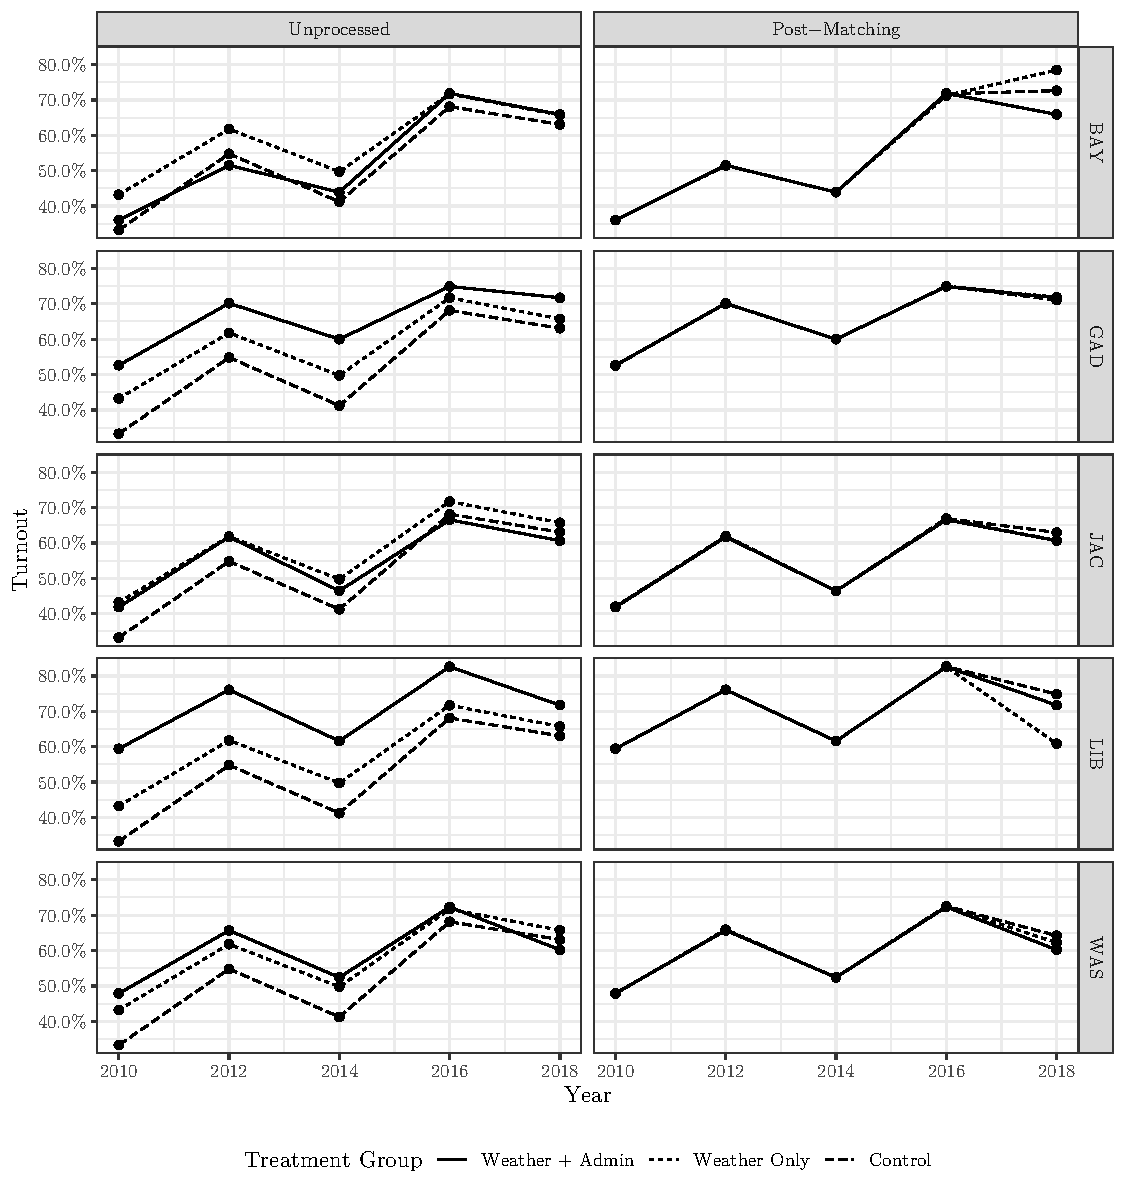
\includegraphics{si_files/figure-latex/indcs-chunk-tr-1} 

}

\caption{\label{fig:ind-counties-tri}Pre- and Post-Matching County Plots}\label{fig:indcs-chunk-tr}
\end{figure}

Figure \ref{fig:ind-counties-tri} presents visual corroboration for what we find in the body of the paper---namely, that counties with more closures saw negative administrative treatment effects. The negative administrative treatment in Bay County is clearly quite large, while the positive administrative treatment effect is clear for Liberty County. Somewhat surprisingly, the weather-only matched voters for Bay County saw substantially higher turnout in 2018 relative to the controls elsewhere in the state; however, as discussed in the body of this paper, the weather was relatively mild at the edges of Bay County. In each county, the matching procedure substantially improves the reasonableness of the parallel trends assumption necessary for valid causal inference.

\hypertarget{multinomial-regression-table}{%
\section*{Multinomial Regression Table}\label{multinomial-regression-table}}
\addcontentsline{toc}{section}{Multinomial Regression Table}

In Figure 5 in the body of the paper, we show the marginal effects plot based on a mulinomial logistic regression. Because those coefficients can be difficult to interpret on their own, we have included the regression table here. While the coefficients have been exponentiated in this table, the standard errors have been left unadjusted.

\begin{singlespace}
\input{"../temp/multinom.tex"}
\end{singlespace}

\hypertarget{references}{%
\section*{References}\label{references}}
\addcontentsline{toc}{section}{References}

\hypertarget{refs}{}
\begin{CSLReferences}{1}{0}
\leavevmode\hypertarget{ref-Caliendo2008}{}%
Caliendo, Marco, and Sabine Kopeinig. 2008. {``Some {Practical Guidance} for the {Implementation} of {Propensity Score Matching}.''} \emph{Journal of Economic Surveys} 22 (1): 31--72. \url{https://doi.org/10.1111/j.1467-6419.2007.00527.x}.

\leavevmode\hypertarget{ref-Hainmueller2012}{}%
Hainmueller, Jens. 2012. {``Entropy {Balancing} for {Causal Effects}: {A Multivariate Reweighting Method} to {Produce Balanced Samples} in {Observational Studies}.''} \emph{Political Analysis} 20 (1): 25--46. \url{https://doi.org/10.1093/pan/mpr025}.

\end{CSLReferences}

\end{document}
